\chapter{Classes}
\label{cap:p1}

Nesta secção apresentam-se as classes usadas. Tanto o motor como o gerador recorrem extensivamente a estas classes para desempenhar as suas funções. Algumas destas classes são recorrentes e usadas mais que uma vez em diferentes contextos. Assim, antes de introduzir como funciona o motor e o gerador é importante primeiro perceber quais são as classes que ambos usam, bem como a função de cada uma.

O objectivo de construção destas classes foi simplificar a construção do motor e gerador apenas. Nesta primeira etapa, foram deixadas para segundo plano questões como a modularidade e encapsulamento de dados, embora seja algo a considerar em etapas posteriores do trabalho.

\section{Ponto3D}

Tanto o gerador como o motor trabalham com pontos. Assim, foi criada uma classe que representa o conceito de um ponto num espaço 3D:

\begin{Verbatim}
	struct Ponto3D {
		float x, y, z;
	};
\end{Verbatim}

Como se pode verificar, esta classe é bastante simples e apenas contém 3 variáveis do tipo \textit{float}, correspondentes às coordenadas cartesianas de um ponto num espaço 3D.

Visto nenhuma das aplicações exigir operações complexas sobre pontos, esta classe foi mantida simples. De facto, tanto motor como gerador, apenas precisam de ler valores de coordenadas de pontos e ocasionalmente mudar os seus valores, o que pode ser feito directamente acedendo às variáveis desta classe.

O facto desta classe ser simples e não ter nenhuma função ou construtor faz com que seja considerada pelo C++ como uma \textit{aggregate class}. Este tipo de classe tem propriedades específicas, nomeadamente uma inicialização fácil e intuitiva das instâncias, o que contribui também para código mais fácil de ler. Esse fator foi fundamental para a decisão de manter a classe simples.

\newpage
\section{CoordsPolares}
\label{p1:coordsPolares}
Esta classe pretende abstrair os cálculos relacionados com coordenadas polares. A ideia é poderem ser criadas instâncias desta classe indicando os parâmetros correspondentes a coordenadas polares e as correspondentes coordenadas cartesianas poderem ser obtidas facilmente a partir da instância.

As coordenadas polares são constituídas por um ponto central, um raio e por um ângulo $\alpha$ (também designado por ângulo azimuth) e permitem localizar um ponto num plano conforme se ilustra na figura \ref{p1:fig:p1_polarCoords}:

\begin{figure}[<+htpb+>]
	\centering
	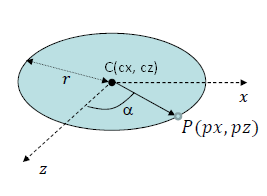
\includegraphics[scale=1.0]{imagens/p1_polarCoords.png}
	\caption{Localização de um ponto P(px,py,pz) segundo um centro C(cx,cy,cz), um ângulo azimuth ($\alpha$) e um raio $r$}
	\label{p1:fig:p1_polarCoords}
\end{figure}

Designando o ponto central como C(cx,cy,cz) e um ponto P(px,py,pz) que se pretende localizar, temos que as coordenadas px e py podem ser obtidas da seguinte forma:\\

	$px = cx + r \times sin(\alpha)$
	
	$py = cy$
	
	$pz = cz + r \times cos(\alpha)$\\

A classe \textit{CoordsPolares} representa apenas uma forma fácil de trabalhar com este sistema de coordenadas. Esta classe possui variáveis de instância relacionadas com as suas coordenadas polares e cartesianas:

\begin{Verbatim}
	//Centro a partir do qual se 
	//considera as coordenadas polares
	Ponto3D centro;
	//Coordenadas polares
	float raio, azimuth;
	//Coordenadas rectangulares correspondentes 
	//às coordenadas polares
	Ponto3D cCartesianas;
\end{Verbatim}

O ponto chave desta classe é que as variáveis das coordenadas polares e cartesianas referem-se sempre ao mesmo ponto. Sempre que um dos parâmetros é alterado (através de uma das funções disponibilizadas), todos os restantes são actualizados em conformidade.

A classe tem um único construtor:

\begin{Verbatim}
CoordsPolares(Ponto3D c, float r, float az);
\end{Verbatim}

Neste construtor são pedidos os parâmetros referentes às coordenadas polares. O primeiro parâmetro \textit{c} corresponde ao ponto central, o segundo parâmetro r corresponde ao raio e o último parâmetro corresponde ao ângulo azimuth ($\alpha$). Ao receber estas coordenadas polares, o construtor seguidamente atualiza as variáveis de instância em conformidade, nomeadamente coloca na variável de instância \textit{cCartesianas} as coordenadas cartesianas correspondentes às coordenadas polares passadas como argumento. Essa actualização é feita pela função \textit{refreshCartesianas()}:

\begin{Verbatim}
void refreshCartesianas(){
	cRectangulares.x = centro.x + raio * sin(azimuth);
	cRectangulares.y = centro.y;
	cRectangulares.z = centro.z + raio * cos(azimuth);
}
\end{Verbatim}

Como se pode ver, esta função implementa apenas as fórmulas apresentadas anteriormente. Esta função é privada à classe, por isso não pode ser chamada em qualquer parte do código. É a própria classe que se responsabiliza por chamar esta função sempre que necessário.

Assim, dada uma instância desta classe é sempre possível saber as coordenadas cartesianas correspondentes através da função \textit{toCartesianas()}:

\begin{Verbatim}
Ponto3D toCartesianas() {
	return cCartesianas;
}
\end{Verbatim}


\section{CoordsEsfericas}
\label{p1:cEsfericas}
Esta classe pretende abstrair os cálculos relacionados com coordenadas esféricas. A ideia é poderem ser criadas instâncias desta classe indicando os parâmetros correspondentes a coordenadas esféricas e as correspondentes coordenadas cartesianas poderem ser obtidas facilmente a partir da instância. É também possível fazer o inverso, ou seja, indicar um ponto com coordenadas cartesianas e obter as respectivas coordenadas esféricas.

As coordenadas esféricas são constituídas por um raio $r$, por um ângulo $\theta$ (também designado por ângulo azimuth) e um ângulo $\phi$ (também designado por ângulo polar), conforme apresentado na figura \ref{p1:fig:p1_sphericalCoords}:

\begin{figure}[<+htpb+>]
	\centering
	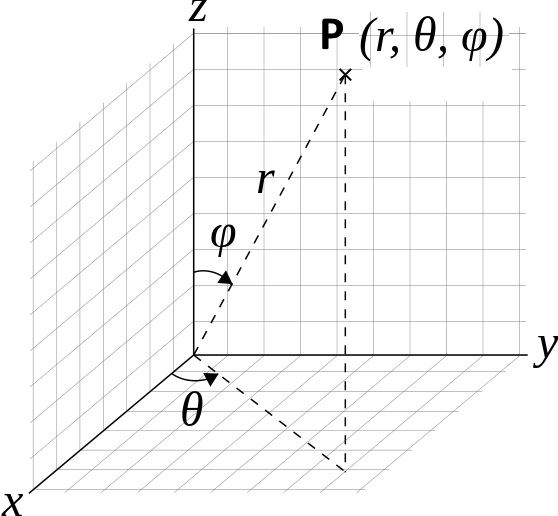
\includegraphics[scale=0.5]{imagens/p1_sphericalCoords.png}
	\caption{Localização de um ponto P segundo coordenadas esféricas}
	\label{p1:fig:p1_sphericalCoords}
\end{figure}

É possível saber as coordenadas cartesianas de um ponto P(px,py,pz) a partir das suas coordenadas esféricas através das seguintes fórmulas:\\

		$px = r \times cos(\theta) \times sin(\phi)$
		
		$py = r \times sin(\theta) \times sin(\phi) $
		
		$pz = r \times cos(\phi)$\\


Por outro lado, consegue-se saber também as coordenas esféricas de um ponto a partir das suas coordenadas cartesianas de acordo com as seguintes fórmulas:\\

		$r = \sqrt{px^2 + py^2 + pz^2}$
		
		$\theta = \arctan(py \backslash px) $
		
		$\phi = \arccos (pz \backslash r)$\\

De referir que ao contrário da classe \textit{CoordsPolares}, nesta classe optou-se por não se considerar um centro. Assume-se o centro como sendo (0.0,0.0,0.0) sempre. Considerou-se esta simplificação razoável na medida em que responde aos requisitos do motor e gerador nesta primeira fase.

A classe \textit{CoordsEsfericas} tem as seguintes variáveis de instância:

\begin{Verbatim}
// Coordenadas Esfericas
float raio, azimuth_ang, polar_ang;
// Coordenadas cartesianas
Ponto3D cCartesianas;
\end{Verbatim}

O ponto chave desta classe é que as variáveis das coordenadas esféricas e cartesianas referem-se sempre ao mesmo ponto. Sempre que um dos parâmetros é alterado (através de uma das funções disponibilizadas), todos os restantes são atualizados em conformidade.

Uma instância da classe \textit{CoordsEsfericas} pode ser criada indicando os parâmetros das coordenadas esféricas (para se saber as suas coordenadas cartesianas), ou indicando um ponto em coordenadas cartesianas (do qual se pretende saber as coordenadas esféricas), através dos seguintes construtores:

\begin{Verbatim}
CoordsEsfericas(float r, float az, float polar);
CoordsEsfericas(Ponto3D pto);
\end{Verbatim}

Caso a instância seja criada a partir de coordenadas polares, o construtor calcula as coordenadas cartesianas correspondentes através da função \textit{refreshCartesianas()}:

\begin{Verbatim}
void refreshCartesianas() {
	cCartesianas.z = raio * sin(polar_ang) * cos(azimuth_ang);
	cCartesianas.x = raio * sin(polar_ang) * sin(azimuth_ang);
	cCartesianas.y = raio * cos(polar_ang);
}
\end{Verbatim}

Caso a instância seja criada a partir de coordenadas cartesianas, o construtor calcula as coordenadas polares correspondentes através da função \textit{refreshEsfericas()}:

\begin{Verbatim}
void refreshEsfericas() {
	raio = sqrt(pow(cCartesianas.x, 2) + 
		pow(cCartesianas.y, 2) + 
		pow(cCartesianas.z, 2));
	polar_ang = acos(cCartesianas.y / raio);
	azimuth_ang = atan2(cCartesianas.x, cCartesianas.z);
}
\end{Verbatim}

Estas duas funções correspondem à implementação das fórmulas apresentadas anteriormente e garantem que as variáveis de instância correspondentes às coordenadas esféricas e cartesianas se referem sempre ao mesmo ponto. Ambas são funções privadas, pelo que é a própria classe que tem a responsabilidade de as chamar sempre que é necessário atualizar valores.

A qualquer momento, é possível saber as coordenadas cartesianas de uma instância pela função \textit{toCartesianas()}

\begin{Verbatim}
Ponto3D toCartesianas() {
	return cCartesianas;
}
\end{Verbatim}

Além destas funções, a classe possui ainda funções adicionais que permitem mudar a posição do ponto representado por cada instância. Sempre que uma destas funções é chamada tanto as variáveis de instância das coordenadas polares e cartesianas são atualizadas quer pela função refreshEsfericas() ou refreshCartesianas(). Estas funções que permitem mudar a localização do ponto, garantem ainda que $0 \leq \phi \leq \pi$ e que $0 \leq \theta \leq 2 \times \pi$

\newpage

\section{Figura}

Esta classe representa uma figura que será desenhada pelo motor. Representa por isso apenas um conjunto de pontos numa determinada ordem que correspondem a triângulos, que por sua vez formam uma figura.

Por representar um conjunto de pontos, sem surpresa, a sua única variável de instância é um vector de pontos:

\begin{Verbatim}
std::vector<Ponto3D> pontos;
\end{Verbatim}

A utilidade desta classe revela-se pelas funções que disponibiliza. Em primeiro lugar, disponibiliza um conjunto de funções que quando chamadas colocam no vector \textit{pontos} os pontos necessários para o desenho de uma figura em concreto. Dessa forma, estas funções permitem criar planos, caixas, círculos, cilindros e esferas. Estas funções serão explicadas em mais detalhe quando for apresentado o gerador onde será mostrado de que forma estas funções podem ser chamadas bem como de que forma geram os pontos.

Além das funções que permitem criar figuras destaca-se ainda a função \textit{toFicheiro()}, que permite guardar os pontos da figura num ficheiro cujo nome é passado como argumento.

\begin{Verbatim}
void toFicheiro(std::string filePath)
\end{Verbatim}

É ainda possível obter os pontos da figura pela função \textit{getPontos()}:

\begin{Verbatim}
std::vector<Ponto3D> getPontos()
\end{Verbatim}

\section{TinyXML-2}

Esta biblioteca foi usada para auxílio à leitura de ficheiros XML por parte do motor e pode ser encontrada no endereço: http://www.grinninglizard.com/tinyxml2/
